\documentclass[11pt,a4paper]{article}

\usepackage[margin=2.0cm,top=2.2cm,bottom=2.2cm]{geometry}
\usepackage{amsmath,amssymb,amsthm}
\allowdisplaybreaks
\usepackage{enumitem}
\usepackage{booktabs}
\usepackage{graphicx}
\usepackage{float}
\usepackage{placeins}
\usepackage{xcolor}
\usepackage[colorlinks=true, linkcolor=blue!45!black, urlcolor=blue!45!black, citecolor=blue!45!black]{hyperref}
\usepackage{parskip}
\usepackage{fancyhdr}

\setlength{\headheight}{13.6pt}
\pagestyle{fancy}
\fancyhf{}
\lhead{Computational Genomics}
\rhead{Exercise 2}
\cfoot{\thepage}
\renewcommand{\headrulewidth}{0.4pt}

\newcommand{\E}{\mathbb{E}}
\newcommand{\Var}{\mathrm{Var}}
\newcommand{\Pois}{\mathrm{Poisson}}
\newcommand{\Ind}[1]{\mathbf{1}\{#1\}}
\newcommand{\hlam}{\hat{\lambda}}
\newcommand{\hM}{\hat{M}}
\newcommand{\Nsub}{N_{\mathrm{sub}}}
\newcommand{\Uobs}{U_{\mathrm{obs}}}
\newcommand{\TVD}{\mathrm{TVD}}

\begin{document}

\begin{center}
    {\Large\bfseries Computational Genomics -- Exercise 2}

    \vspace{0.4em}
    {\large Library Complexity}

    \vspace{0.7em}
    Roee Tekoah \quad
    (\href{mailto:roee.tekoah@mail.huji.ac.il}{roee.tekoah@mail.huji.ac.il})
\end{center}

\vspace{0.4em}

\setcounter{tocdepth}{2}
\begingroup
\renewcommand{\contentsname}{\normalsize Contents}
{\small\tableofcontents}
\endgroup

\vspace{0.4em}

\section{Setup and notation}

\paragraph{Supplementary material.}
Two short primers accompany this submission as background material I wrote
while working through the unfamiliar parts of the exercise:
\texttt{subsampling\_primer.pdf} (the Heck rarefaction / Monte Carlo
subsampling estimator used in Q2(a)) and \texttt{stats\_primer.pdf} (the
chi-squared goodness-of-fit, Wilks' dof correction, and the per-bin LRT
used in Q2(b) and Q3(b)). They are cited from the relevant sections below;
the main report is self-contained without them.

\paragraph{A note on notation.}
\texttt{Ex2.pdf} and the Lecture~10 notes use inconsistent symbols (notably, $N$
and $M$ are swapped). This report uses the \textbf{Lecture~10 convention}
throughout; mapping:

\begin{center}
\renewcommand{\arraystretch}{1.15}
\begin{tabular}{lll}
\textbf{Quantity} & \textbf{Ex2.pdf} & \textbf{This report (Lecture 10)} \\\hline
True \# molecules in the library (complexity)  & $N$              & $M$ \\
\# sequenced reads                              & $M$              & $N$ \\
\# unique molecules observed                    & $M_u$            & $U$ \\
Per-molecule read count                         & $k_i$            & $n_j$ \\
Rate per molecule                               & $\lambda = M/N$  & $\lambda = N/M$ \\
\end{tabular}
\end{center}

\paragraph{Model and identities.}
Each of the $M$ original molecules has a unique sequence (deduplication recovers $U$
exactly), and per-molecule read counts are i.i.d.\ $n_j \sim \Pois(\lambda)$
($j=1,\dots,M$), with $N = \sum_j n_j$ and $U = \sum_j \Ind{n_j > 0}$. Intuitively,
$\lambda$ is the average number of reads each molecule receives -- bigger $\lambda$ means
deeper effective sequencing per molecule. Following Ex2.pdf, $\lambda$ is kept as a
free parameter (needed in Q3). Immediate consequences:
$\Pr(n_j > 0) = 1 - e^{-\lambda}$,\;
$\E[U] = M(1 - e^{-\lambda})$ (the library-saturation curve, linear at small
$\lambda$, capped at $M$ as $\lambda \to \infty$; see
Figure~\ref{fig:saturation}),\; $\E[N] = \lambda M$,\; and
$\E[U]/\E[N] = (1 - e^{-\lambda})/\lambda$.

\begin{figure}[!htbp]
\centering
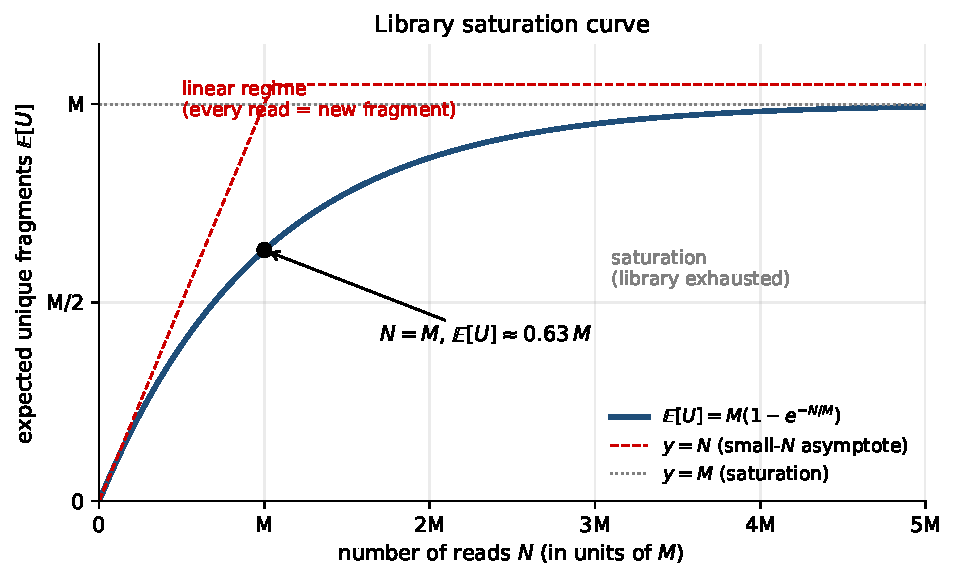
\includegraphics[width=0.75\linewidth]{fig1_saturation.pdf}
\caption{Saturation curve $\E[U] = M(1 - e^{-N/M})$. Linear for $N \ll M$, capped at
$M$ for $N \gg M$. At $N = M$, $\E[U] \approx 0.63\,M$.}
\label{fig:saturation}
\end{figure}

\paragraph{Procedure from the Setup.}
Substituting observed for expected, then solving for $\hlam$ and $\hM$:
\[
   \frac{U}{N} \;\approx\; \frac{1 - e^{-\lambda}}{\lambda}
   \quad\Longrightarrow\quad
   \hM \;\approx\; \frac{U}{1 - e^{-\hlam}} \;=\; \frac{N}{\hlam}.
\]
$\hlam$ is solved numerically from the first equation. The two forms of $\hM$
on the right are equal by direct rearrangement of that equation: multiplying
$\hlam/(1-e^{-\hlam}) = N/U$ by $U/\hlam$ gives $U/(1-e^{-\hlam}) = N/\hlam$.

\section{Question 1 -- Maximum-likelihood estimator for \texorpdfstring{$\lambda$}{lambda}}

\subsection{(a) The observation likelihood $P_{\mathrm{obs}}(n_j;\lambda)$}
\emph{Question (Ex2.pdf).} What is $P_{\mathrm{obs}}(k_i;\lambda)$? Hint: if
$k_i = 0$ the molecule is not observed and we do not know it exists.

The model has $n_j \sim \Pois(\lambda)$, but the plain Poisson mass function
$P(n_j;\lambda)$ does not suffice on its own: $P_{\mathrm{obs}}$ must condition
on $n_j > 0$, since we do not observe molecules with $n_j = 0$ -- they are
invisible to us. Therefore:
\begin{align*}
L(\lambda)
  &= \prod_{j\,:\,n_j > 0} P_{\mathrm{obs}}(n_j;\lambda)
   = \prod_{j\,:\,n_j > 0} P(n_j ;\, \lambda,\, n_j > 0) \\
  &\overset{\text{cond.\ prob.}}{=}
     \prod_{j\,:\,n_j > 0} \frac{P_\lambda(n_j,\, n_j > 0)}{P_\lambda(n_j > 0)}
   \;\overset{\{n_j=k\}\,\subseteq\,\{n_j>0\}}{=}\;
     \prod_{j\,:\,n_j > 0} \frac{P_\lambda(n_j)}{1 - P_\lambda(n_j = 0)} \\
  &= \prod_{j\,:\,n_j > 0} \frac{\,e^{-\lambda}\, \dfrac{\lambda^{n_j}}{n_j!}\,}{1 - e^{-\lambda}}.
\end{align*}

\subsection{(b) Log-likelihood and sufficient statistics}
\emph{Question (Ex2.pdf).} Write the analytical form of the (log-)likelihood.
What are the sufficient statistics?

From (a), $L(\lambda) = \prod_{j\,:\,n_j > 0} \dfrac{e^{-\lambda}\, \lambda^{n_j}/n_j!}{1 - e^{-\lambda}}$. Taking the log:
\begin{align*}
\ell(\lambda) \;:=\; \log L(\lambda)
  &= \sum_{j\,:\,n_j > 0} \log\!\left( \frac{\,e^{-\lambda}\, \dfrac{\lambda^{n_j}}{n_j!}\,}{1 - e^{-\lambda}} \right) \\
  &= \sum_{j\,:\,n_j > 0} \Bigl[\, \log(e^{-\lambda}) + \log(\lambda^{n_j}) - \log(n_j!) - \log(1 - e^{-\lambda}) \,\Bigr] \\
  &= \sum_{j\,:\,n_j > 0} \Bigl[\, -\lambda + n_j \log(\lambda) - \log(n_j!) - \log(1 - e^{-\lambda}) \,\Bigr].
\end{align*}
Since $\lambda$ is the unknown parameter, the minimal sufficient statistic for
$\lambda$ is the pair $(U,\,N)$ with $U = \#\{j : n_j > 0\}$ and
$N = \sum_{j : n_j > 0} n_j$. (The full vector $\{n_j : n_j > 0\}$ is trivially
sufficient too, but the factorisation in (c) shows the meaningful compression.)

\subsection{(c) Solving for $\hlam = \arg\max_\lambda L(\lambda)$}
\emph{Question (Ex2.pdf).} How would you solve for $\hat\lambda = \arg\max_\lambda L(\lambda)$?

Since $\log$ is monotonic, $\hlam = \arg\max_\lambda L(\lambda) = \arg\max_\lambda \ell(\lambda)$.
Starting from (b), drop $\log(n_j!)$ (no $\lambda$-dependence) and split the sum
term-by-term, pulling constants out of each:
\begin{align*}
\hlam
  &= \arg\max_{\lambda > 0}\;
     \sum_{j\,:\,n_j > 0} \Bigl[\, -\lambda + n_j \log(\lambda) - \log(1 - e^{-\lambda}) \,\Bigr] \\
  &= \arg\max_{\lambda > 0}\;
     \Biggl\{\, \sum_{j\,:\,n_j>0}(-\lambda)
              + \log(\lambda)\!\!\sum_{j\,:\,n_j>0}\! n_j
              + \sum_{j\,:\,n_j>0}\!\bigl(-\log(1 - e^{-\lambda})\bigr) \,\Biggr\} \\
  &= \arg\max_{\lambda > 0}\;
     \Bigl\{\, -U\lambda + N \log(\lambda) - U \log(1 - e^{-\lambda}) \,\Bigr\}
     && \text{(with $U = \#\{j : n_j > 0\}$, $N = \sum_j n_j$).}
\end{align*}
Differentiating w.r.t.\ $\lambda$ (chain rule on the last term):
\begin{align*}
\frac{d}{d\lambda}\Bigl[\,-U\lambda + N \log(\lambda) - U \log(1 - e^{-\lambda})\,\Bigr]
  &= -U + \frac{N}{\lambda} - U \cdot \frac{1}{1 - e^{-\lambda}} \cdot \frac{d}{d\lambda}\bigl(1 - e^{-\lambda}\bigr) \\
  &= -U + \frac{N}{\lambda} - U \cdot \frac{e^{-\lambda}}{1 - e^{-\lambda}}.
\end{align*}
Set this to zero at $\lambda = \lambda^{\ast}$, then gather the $U$ terms before
isolating $\lambda^{\ast}$:
\begin{align*}
-U + \frac{N}{\lambda^{\ast}} - U \cdot \frac{e^{-\lambda^{\ast}}}{1 - e^{-\lambda^{\ast}}}
  &\;=\; 0 \\
\frac{N}{\lambda^{\ast}}
  &\;=\; U + U \cdot \frac{e^{-\lambda^{\ast}}}{1 - e^{-\lambda^{\ast}}}
     && \text{(move both $U$-terms to the right)} \\
  &\;=\; U\!\left( 1 + \frac{e^{-\lambda^{\ast}}}{1 - e^{-\lambda^{\ast}}} \right)
     && \text{(factor $U$)} \\
  &\;=\; U \cdot \frac{1 - e^{-\lambda^{\ast}} + e^{-\lambda^{\ast}}}{1 - e^{-\lambda^{\ast}}}
     && \text{(common denominator)} \\
  &\;=\; \frac{U}{1 - e^{-\lambda^{\ast}}}
     && \text{(numerator $= 1$)} \\
\Longrightarrow\quad
   & \boxed{\;\dfrac{\lambda^{\ast}}{1 - e^{-\lambda^{\ast}}} \;=\; \dfrac{N}{U}\;}
     && \text{(multiply both sides by $\lambda^{\ast}\!/U$).}
\end{align*}
This is identical to the equation $U/N = (1 - e^{-\lambda})/\lambda$ from the
Setup: the MLE and the Setup procedure coincide here. The equation has no
closed form, so solve numerically by finding the root of
\[
   g(\lambda) \;=\; \frac{\lambda}{1 - e^{-\lambda}} - \frac{N}{U},
\]
e.g.\ by Newton's method, bisection, or fixed-point iteration.

\subsection{(d) Estimating $M$ given $\hlam$}
\emph{Question (Ex2.pdf).} Once you estimate $\hat\lambda$, what is the
estimate of $N$? (Ex2's $N$ = our $M$, the library complexity.)

The MLE equation in (c) gives $\hlam/(1 - e^{-\hlam}) = N/U$, which alone only
reproduces the \emph{observed} count $U$, not the true library complexity $M$.
To estimate $M$, applying the Setup substitution
$U \approx \E[U] = M\bigl(1 - e^{-\hlam}\bigr)$ gives
\[
   \hM \;\approx\; \frac{U}{1 - e^{-\hlam}} \;=\; \frac{N}{\hlam},
\]
where the second equality is the same rearrangement of the MLE equation as in
the Setup. This matches the Setup procedure exactly.

\section{Question 2 -- Estimating \texorpdfstring{$\lambda$}{lambda} on the supplied data}

\paragraph{Files.}
The four supplied files are \texttt{Sample1\_pt1}, \texttt{Sample1\_pt2},
\texttt{Sample1\_pt3}, and \texttt{Sample2}. Each row of a file is a tuple
$(\mathrm{chr},\mathrm{start},\mathrm{end},n_j)$ with $n_j \geq 1$. From each file
we compute $U = \#\{\text{rows}\}$ and $N = \sum_j n_j$.

\paragraph{What ``procedure discussed in class'' means here.}
The exercise's single-equation estimator $U/N = (1 - e^{-\lambda})/\lambda$
is algebraically the same as the equation we get from $\partial\ell/\partial\lambda
= 0$ in Q1(c) (cross-multiply), so a direct comparison is vacuous. The substantive comparison must be against the lecture's
library-complexity estimator -- a subsampled curve fit of
$\E[U] = M(1 - e^{-N/M})$ -- which is a different procedure and gives a generally
different $\hM$. I take that as the intended comparison.

\begin{figure}[!htbp]
\centering
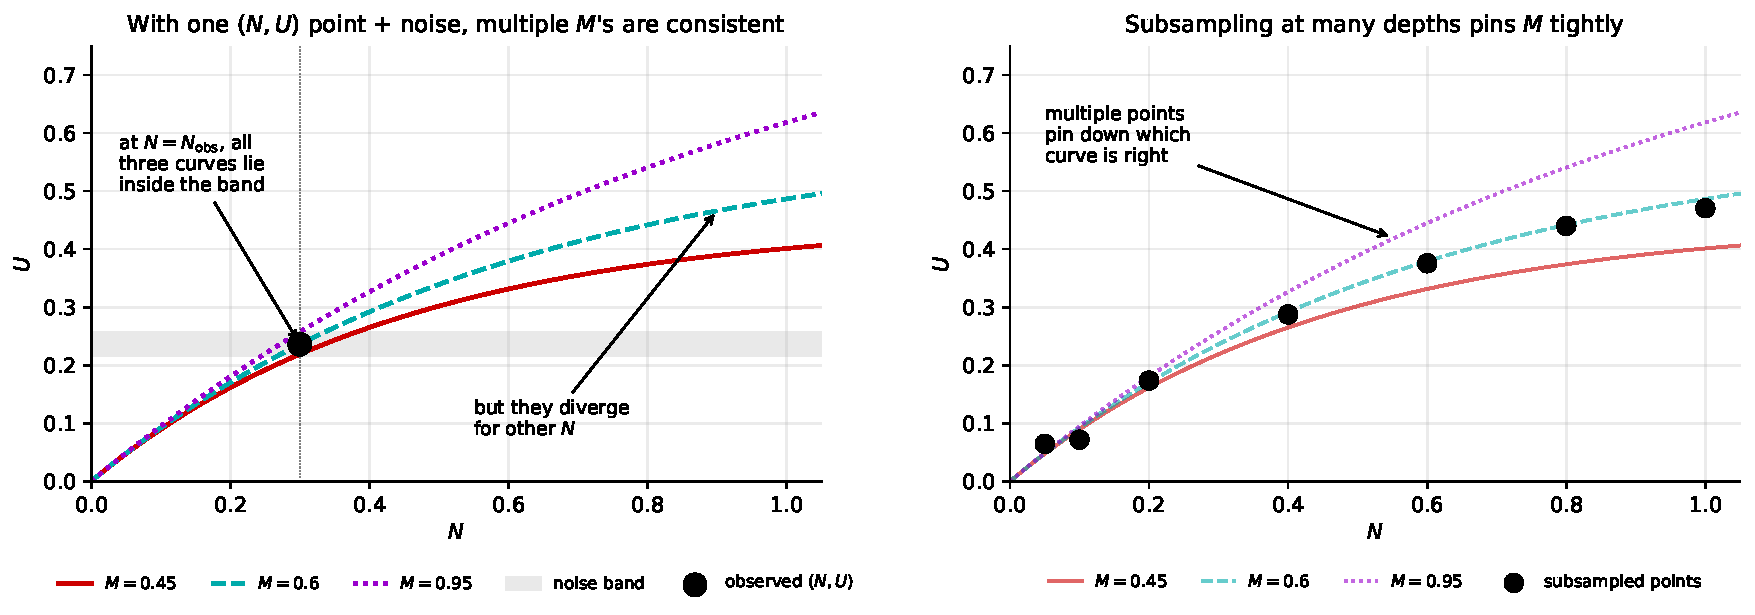
\includegraphics[width=\linewidth]{fig2_ambiguity.pdf}
\caption{Why the subsampling approach is more informative than the single-point
estimator. \textbf{Left:} a single observed $(N, U)$ point with a noise band; three
different values of $M$ all give predictions inside the band at $N = N_{\mathrm{obs}}$
-- the single point cannot tell us which curve generated the data. \textbf{Right:}
multiple subsampled $(N_{\mathrm{sub}}, U_{\mathrm{obs}})$ points pick out the correct
curve unambiguously.}
\label{fig:q2-motivation}
\end{figure}

\subsection{(a) Q1 MLE vs.\ subsampling curve-fit on each file}
\emph{Question (Ex2.pdf).} Estimate $\hat\lambda$ using both the procedure
discussed in class and the maximum likelihood method derived in Q1, on each
file. How do the two estimates differ?

Both estimators are run on each file: the Q1 MLE (single-point root-find) and the
subsampling curve fit (multi-point least squares).

\subsubsection*{Method 1: Q1 MLE (single-point root-find)}

For each file, $\hlam$ solves
\[
   g(\lambda) \;=\; \dfrac{\lambda}{1 - e^{-\lambda}} - \dfrac{N}{U} \;=\; 0,
\]
and the library-complexity estimate is $\hM_{\text{MLE}} = N / \hlam$. The function
$g$ is continuous and strictly increasing on $(0,\infty)$, with
$g(0^{+}) = 1 - N/U \leq 0$ (since $N \geq U$) and $g(\lambda) \to +\infty$ as
$\lambda \to \infty$, so it has a unique positive root.

\paragraph{Numerical method.}
I use \texttt{scipy.optimize.brentq}, a bracketed 1D root finder (a hybrid of
bisection and inverse-quadratic interpolation; both bisection and the IVT it
relies on were covered in Infi~1). The bracket is $[10^{-10},\, N/U]$: at the
lower end $g(0^{+}) = 1 - N/U \le 0$ (since $N \ge U$), and at the upper end
$g(N/U) = (N/U)\,e^{-N/U}/(1 - e^{-N/U}) > 0$ unconditionally, so the IVT
guarantees a root in between. Newton would have worked too but needs a derivative
and a good starting point; brentq doesn't.

\subsubsection*{Method 2: Subsampling curve fit (multi-point least squares)}

For each file I generate $(\Nsub, \Uobs)$ pairs at depth fractions
$d \in \{0.05,\, 0.1,\, 0.2,\, 0.4,\, 0.6,\, 0.8,\, 1.0\}$, then fit $M$ to the
saturation curve through those points.

\paragraph{Producing the $(\Nsub, \Uobs)$ points: Monte Carlo subsampling.}
For each depth fraction $d$, randomly pick $m = \lfloor dN \rfloor$ reads without
replacement from the bag of $N$ reads, then count how many distinct fragments are
present. Each trial is one independent random draw; averaging over $5$ seeds
reduces sampling noise like $\mathcal{O}(1/\sqrt{\text{trials}})$ by the
standard-error-of-the-mean argument.\footnote{For i.i.d.\ trials $X_i$ with
finite variance $\sigma^2$, $\Var(\bar X_n) = \sigma^2/n$, so the s.e.\ of the
sample mean shrinks as $1/\sqrt{n}$ (CLT; see e.g.\ Casella \& Berger,
\emph{Statistical Inference}, \S5.2).}

\paragraph{Efficient implementation.}
Instead of materialising a flat $N$-element ticket array (wasteful at
$N \sim 4 \times 10^{6}$), I draw per-fragment counts independently:
$\mathrm{count}_j \sim \mathrm{Hypergeometric}(N, n_j, m)$. The marginals are exact,
the joint is slightly relaxed (independent draws do not enforce
$\sum_j \mathrm{count}_j = m$), but
$\E[\Uobs] = \sum_j \Pr(\mathrm{count}_j > 0)$ depends only on the marginals, so
the estimator is unbiased.

\paragraph{Bonus: closed-form Heck rarefaction.\protect\footnote{Full derivation
of the subsampling/Heck framework and pedagogical figures in the supplementary
\emph{subsampling primer} (\texttt{subsampling\_primer.pdf}).}}
The same expectation has a closed form ($\Pr(\text{miss }j) = \binom{N-n_j}{s}/\binom{N}{s}$;
sum the complement):
\begin{equation}
   \E\!\left[\Uobs(s)\right] \;=\;
   \sum_{j=1}^{U} \!\left[\, 1 - \frac{\binom{N - n_j}{s}}{\binom{N}{s}} \,\right],
   \label{eq:heck-q2}
\end{equation}
computed in log-space via \texttt{scipy.special.gammaln}. I plot it alongside MC in
Figure~\ref{fig:q2-saturation} as an independent check.

\paragraph{Fitting $M$ to the curve.}
Given the $K = 7$ points $(\Nsub^{(i)}, \Uobs^{(i)})$, I minimise the sum of squared
residuals
\[
   \hM_{\text{fit}} \;=\; \arg\min_{M > 0}\; \sum_{i=1}^{K}
   \Bigl(\, \Uobs^{(i)} - M\bigl(1 - e^{-\Nsub^{(i)}/M}\bigr) \,\Bigr)^2.
\]
This is a one-parameter bounded optimisation. I use
\texttt{scipy.optimize.minimize\_scalar} with bounded Brent's method (the 1D
minimisation analogue of \texttt{brentq}), bracketing $M$ between $\max_d \Uobs(dN)$
(the saturation asymptote forces $M \geq \max_d \Uobs$) and a generous ceiling.
\subsubsection*{Numerical results}

The following table combines the Q1 MLE / single-point estimate with the two
curve-fit implementations (Heck rarefaction, exact in expectation; and Monte Carlo,
averaged over 5 random seeds). The last column reports the inflation ratio
$\hM_{\text{MLE}} / \hM_{\text{fit}}$.

\begin{center}
\renewcommand{\arraystretch}{1.2}
\begin{tabular}{lrrrrrrr}
\textbf{File} & \textbf{$N$} & \textbf{$U$} & \textbf{$\hlam$} &
\textbf{$\hM_{\text{MLE}}$} & \textbf{$\hM_{\text{fit (Heck)}}$} &
\textbf{$\hM_{\text{fit (MC)}}$} & \textbf{ratio} \\\hline
Sample1\_pt1 & $1{,}666{,}709$ & $1{,}176{,}492$ & $0.7423$ & $2{,}245{,}206$ & $2{,}218{,}990$ & $2{,}218{,}640$ & $1.0118$ \\
Sample1\_pt2 & $1{,}673{,}083$ & $1{,}133{,}365$ & $0.8370$ & $1{,}998{,}911$ & $1{,}975{,}654$ & $1{,}975{,}235$ & $1.0118$ \\
Sample1\_pt3 & $1{,}094{,}261$ &   $759{,}901$ & $0.7797$ & $1{,}403{,}439$ & $1{,}389{,}006$ & $1{,}389{,}095$ & $1.0104$ \\
Sample2      & $4{,}006{,}586$ & $2{,}332{,}467$ & $1.2008$ & $3{,}336{,}686$ & $3{,}292{,}603$ & $3{,}292{,}292$ & $1.0134$ \\
\end{tabular}
\end{center}

The saturation curves themselves, one per file, are in Figure~\ref{fig:q2-saturation}.

\begin{figure}[!htbp]
\centering
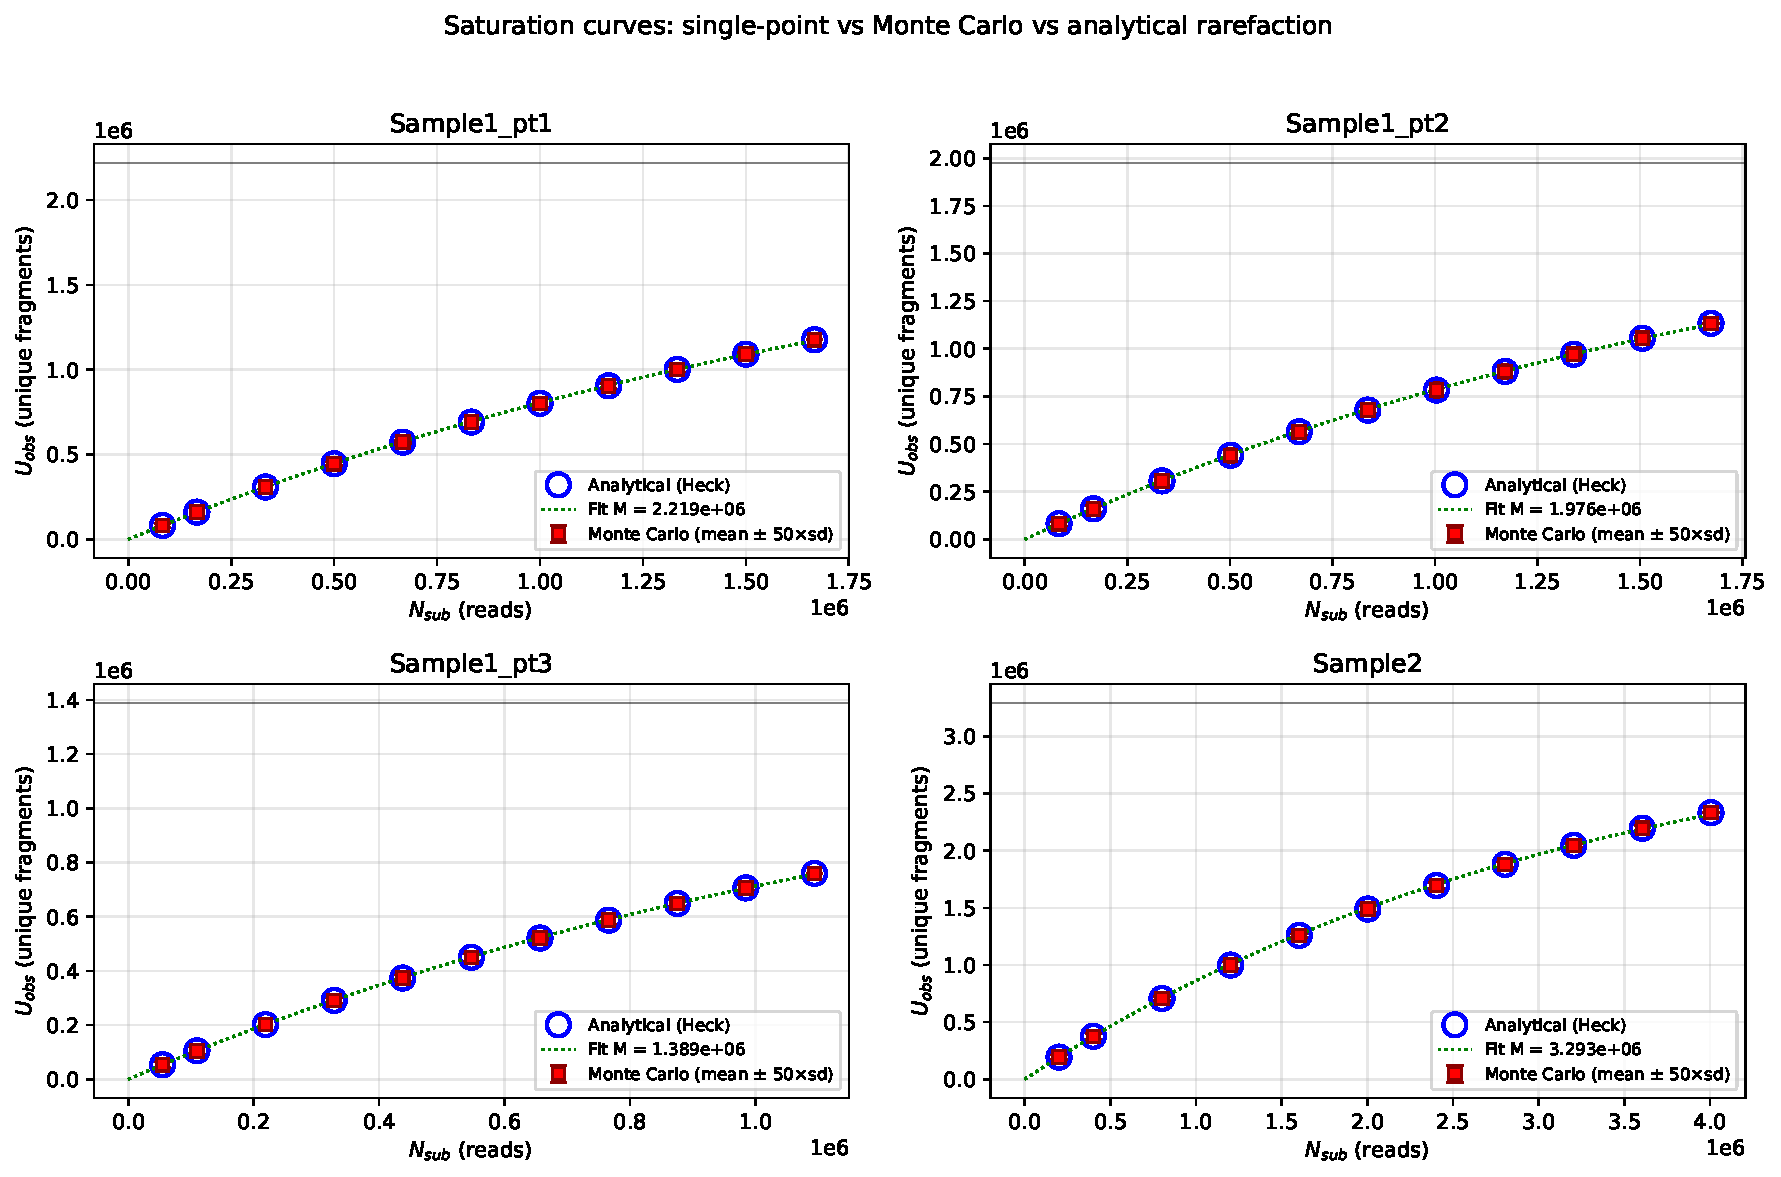
\includegraphics[width=0.92\linewidth]{q2a_saturation.pdf}
\caption{Saturation curves for each file. Analytical rarefaction (blue circles, exact),
Monte Carlo (red squares, mean $\pm$ s.d.\ over 5 trials), and the single-point fit
(green dotted) are plotted against $(\Nsub, \Uobs)$. The thin horizontal line is the
fitted asymptote $\hM_{\text{fit}}$.}
\label{fig:q2-saturation}
\end{figure}

\subsubsection*{Discussion}

\textbf{(i) Monte Carlo agrees with the bonus Heck calculation.}
On every file the MC- and Heck-based $\hM_{\text{fit}}$ agree to within a few
hundred out of millions; Heck~\eqref{eq:heck-q2} is the exact expectation of
the MC procedure, and the residual gap is $\mathcal{O}(1/\sqrt{\text{trials}})$
sampling noise. Both implementations are mutually validated.

\textbf{(ii) MLE vs subsampling fit: agreement with a tell-tale direction.}
$\hM_{\text{MLE}}$ and $\hM_{\text{fit}}$ agree within $1.0$--$1.3\%$ on every
file -- a small surprise that the whole subsampling+Heck+MC+minimiser pipeline
essentially reproduces the one-line single-point root-find. The elaborate fit
pays off only as a diagnostic: the consistent \emph{direction} $\hM_{\text{MLE}}
> \hM_{\text{fit}}$ across four independent files is too systematic for
numerical noise. It signals a model mismatch -- the endpoint $(N,U)$ sits below
where a true uniform-$\lambda$ Poisson curve would put it, forcing the
single-point estimator to inflate $\hM$. Q2(b) tests this; Q3 finds the mechanism.

\textbf{(iii) $\hM$ varies across the three Sample~1 parts.}
$\hM_{\text{fit}} \approx 2.22\text{M}, 1.98\text{M}, 1.39\text{M}$ -- the
largest is $\sim 1.6\times$ the smallest. Library complexity should be a
property of the library, not the depth, so either the three parts are not true
subsamples of one library or the saturation model misses something material.
Sample~2 sits separately with higher $\hlam$ ($\approx 1.20$ vs.\ $0.74$--$0.84$)
and larger $\hM$, consistent with deeper sequencing.

\subsection{(b) Histogram of $n_j$ vs.\ model prediction; goodness-of-fit}
\emph{Question (Ex2.pdf).} Plot the histogram of $n_j$ in each file vs the
model prediction. Do these make sense? Discuss a statistical procedure to
judge whether the observation is surprising under the estimate.

Q2(a) surfaced two pieces of indirect evidence that the uniform-$\lambda$
truncated-Poisson model is misspecified: the systematic $1$--$1.3\%$ inflation
$\hM_{\text{MLE}} > \hM_{\text{fit}}$ on every file, and the $\sim 60\%$ disagreement
on $\hM_{\text{fit}}$ across the three Sample~1 parts. Both point toward
$\lambda$ varying across fragments rather than being a single global rate --
indeed, fitting a single global $\lambda$ is operationally an assumption that
every fragment shares the same per-molecule sequencing rate, which Q3 will show
is false (the $\hlam_\ell$ vary by a factor of $\sim 5$--$10$ with length).
Q2(b) tests that assumption directly: does the empirical histogram of
per-fragment read counts match what the truncated-Poisson at $\hlam$ predicts?

\paragraph{Setup of the test.}
For each file, let $\mathrm{obs}[k] = \#\{j : n_j = k\}$ be the number of observed
fragments with exactly $k$ reads, for $k = 1, 2, \dots, n_{\max}$. Under the Q1 model,
the conditional distribution of $n_j$ given $n_j \geq 1$ is the zero-truncated Poisson
\[
   P_{\mathrm{obs}}(n_j = k \,;\, \lambda)
   \;=\; \dfrac{\,e^{-\lambda}\, \lambda^{k}/k!\,}{1 - e^{-\lambda}},
   \qquad k = 1, 2, 3, \dots
\]
Multiplying by $U$ gives the expected histogram
$\mathrm{exp}[k] = U \cdot P_{\mathrm{obs}}(k \,;\, \hlam)$, i.e.\ the number of the
$U$ observed fragments that should fall in bucket $k$ under the model with
$\lambda = \hlam$.

\paragraph{Statistical procedure: Pearson's chi-squared goodness-of-fit.\protect\footnote{Full
derivation -- variance/CLT chain, $K-1-p$ dof from constraints + Wilks,
Cochran's rule from Poisson-skewness anchors -- in the supplementary
\emph{statistics primer} (\texttt{stats\_primer.pdf}).}}
The right tool for comparing an observed histogram with a parametric model prediction
is the chi-squared goodness-of-fit test. The test statistic is
\[
   \chi^{2} \;=\; \sum_{k}
      \dfrac{\bigl(\mathrm{obs}[k] - \mathrm{exp}[k]\bigr)^{2}}{\mathrm{exp}[k]}.
\]

Under the null hypothesis that the truncated-Poisson model is correct, this
statistic follows approximately the $\chi^{2}$ distribution with $\mathrm{df} =
(\text{number of bins}) - 1 - p$ degrees of freedom: the $-1$ accounts for the
total constraint $\sum \mathrm{obs}[k] = U$ and the $-p$ for parameters estimated
from the data. Here $p = 1$ because $\lambda$ was estimated by MLE from the same
data (the standard Wilks correction\footnote{Not covered in class. See Wilks,
\emph{Ann.\ Math.\ Statist.} 9 (1938) 60--62 for the original asymptotic-$\chi^{2}$
result; also Casella \& Berger, \emph{Statistical Inference}, \S10.3.1.}).

\emph{Cochran tail-merging.}\footnote{Also not covered in class. Cochran,
\emph{Biometrics} 10 (1954) 417--451 -- the canonical reference; modern
statistics texts (e.g.\ Agresti, \emph{Categorical Data Analysis}, \S3.2)
restate it as $\mathrm{exp}[k] \geq 5$ for every bin (some allow $\geq 1$ for a
few bins).} The histogram bins here are the per-fragment read-count
buckets $k = 1, 2, 3, \dots$, not the $5$-bp length bins of Q3. The $\chi^{2}$
approximation requires every bin to have $\mathrm{exp}[k] \geq 5$, otherwise
the discrete sum behaves badly under the continuous $\chi^{2}$. Sparse
right-tail bins (high $k$, where the truncated-Poisson decays exponentially)
routinely fall below this threshold, so I merge from the largest $k$ downwards
into the next bin, accumulating both observed and expected counts, until every
retained bin satisfies $\mathrm{exp}[k] \geq 5$.

\paragraph{Decision rule.}
The $p$-value is
$p\text{-value} = 1 - F_{\chi^{2}}(\chi^{2}_{\text{obs}};\, \mathrm{df})$. A small
$p$-value (say $< 0.05$) means the observed histogram is unlikely under the model,
i.e.\ the uniform-$\lambda$ truncated Poisson is rejected for that file. A large
$p$-value means the model is consistent with the data at the tested level (it does
\emph{not} confirm the model -- absence of evidence is not evidence of absence -- but
it places no constraint on rejection).

\paragraph{Numerical results.}
I run the test with both estimates of $\lambda$ from Q2(a): the single-point MLE
$\hlam_{\text{sp}}$ and the subsampling curve fit $\hlam_{\text{curve}}$ (the latter
is slightly larger, consistent with the smaller $\hM_{\text{fit}}$ from Q2(a) --
$\lambda = N/M$, so smaller $M$ gives larger $\lambda$). Per-file $\chi^{2}$ values:

\begin{center}
\renewcommand{\arraystretch}{1.2}
\begin{tabular}{lrrrr}
\textbf{File} & \textbf{$\hlam_{\text{sp}}$} & \textbf{$\hlam_{\text{curve}}$} &
\textbf{$\chi^{2}_{\text{sp}}$} & \textbf{$\chi^{2}_{\text{curve}}$} \\\hline
Sample1\_pt1 & $0.742$ & $0.751$ & $23{,}911$ & $23{,}111$ \\
Sample1\_pt2 & $0.837$ & $0.847$ & $24{,}529$ & $23{,}659$ \\
Sample1\_pt3 & $0.780$ & $0.788$ & $11{,}402$ & $11{,}094$ \\
Sample2      & $1.201$ & $1.217$ & $54{,}731$ & $53{,}282$ \\
\end{tabular}
\end{center}

After Cochran tail-merging on the per-fragment read-count histogram, every file
retains roughly $5$--$7$ retained bins (collapsing the long sparse right-tail
into a single ``tail'' bin), giving $\mathrm{df} \approx 4$--$6$. This is not
destructive: most of the data sit in the first few low-$k$ bins where the model
already fails egregiously; the tail merge only removes bins with too little
data to test individually. The critical $\chi^{2}_{5}$ at $\alpha = 0.05$ is
$\approx 11.07$; at $\alpha = 10^{-6}$ it is $\approx 32$. The observed values
are in the \emph{tens of thousands}, so $p \approx 0$ at any sensible
threshold. The truncated-Poisson model is rejected on every file regardless of
the dof correction.

Figure~\ref{fig:q2b-hist} shows the four histograms with both prediction curves overlaid.

\begin{figure}[!htbp]
\centering
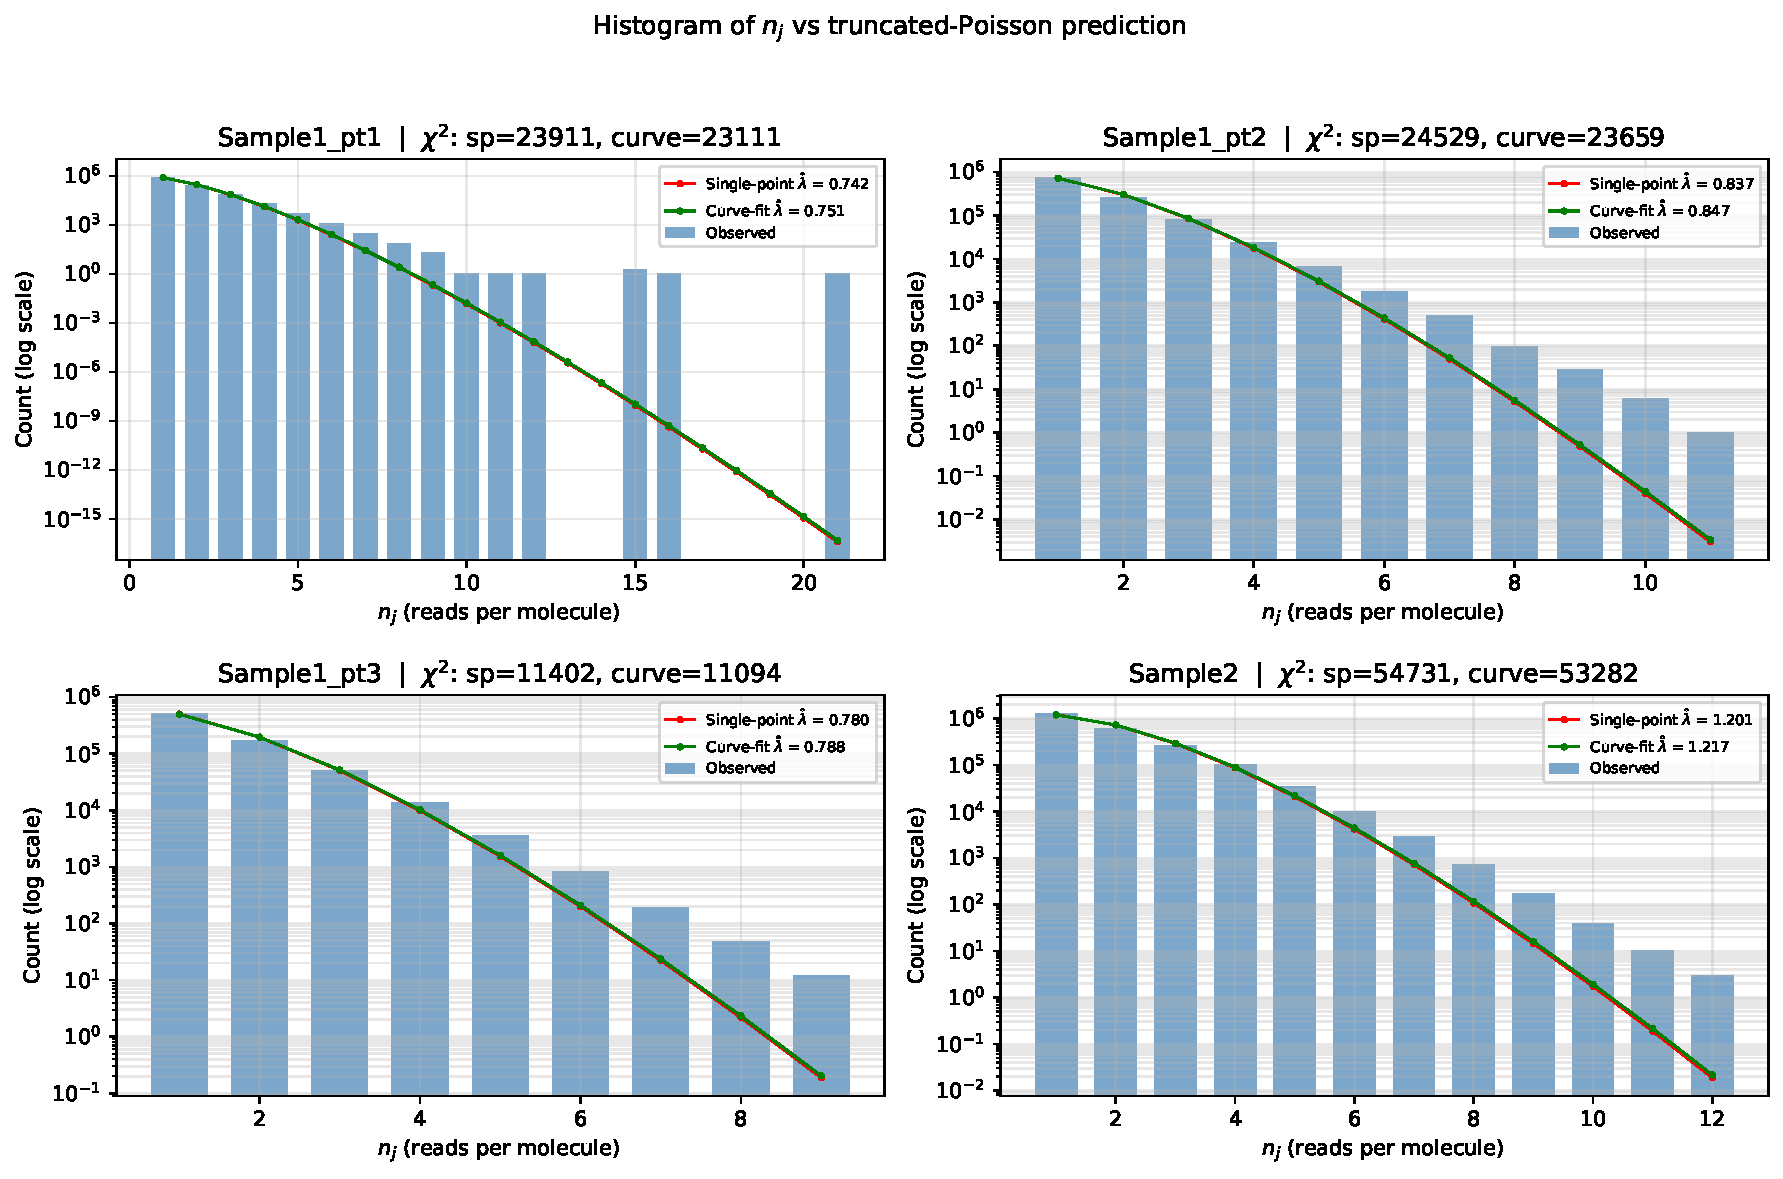
\includegraphics[width=0.78\linewidth]{q2b_histograms.pdf}
\caption{Observed multiplicity histograms (blue bars, log $y$-axis) vs.\ the
zero-truncated Poisson prediction at $\hlam_{\text{sp}}$ (red) and
$\hlam_{\text{curve}}$ (green). The two prediction curves lie essentially on top of
each other because the $\hlam$ values differ by $<1\%$. The bars sit visibly
\emph{above} the curves throughout the right tail on every file, the signature of
heavier-than-Poisson per-fragment counts.}
\label{fig:q2b-hist}
\end{figure}

\paragraph{Discussion.}

\textbf{(i) The two $\hlam$ values give essentially the same $\chi^{2}$.}
$\hlam_{\text{sp}}$ and $\hlam_{\text{curve}}$ are within $\sim 1\%$ (the same
agreement as $\hM$ from Q2(a) by $\hlam = N/\hM$), so the two $\chi^{2}$ columns
agree to a few percent. At this scale of misfit ($\chi^{2} \sim 10^{4}$) the
difference is negligible.

\textbf{(ii) The model has to be rejected outright.}
$\chi^{2}$ in the tens of thousands with $\mathrm{df} \approx 5$ is not
borderline. The failure is visible in Figure~\ref{fig:q2b-hist}: observed bars
overshoot the predicted curve by orders of magnitude in the right tail. The
Q1/Q2(a) chain -- truncated-Poisson likelihood, MLE for $\lambda$, saturation
curve $\E[U] = M(1 - e^{-N/M})$ -- rests on a foundation the data refute, so
$\hlam$ and $\hM$ should be read as descriptive summaries, not ``true''
Poisson rate or library complexity.

\textbf{(iii) The mechanism is heterogeneous $\lambda$, bridging to Q3.}
A heterogeneous-$\lambda$ Poisson model -- each fragment has its own rate
$\lambda_j$ -- can produce arbitrarily heavy right tails: high-$\lambda$
fragments populate the over-represented $n_j \approx 8$--$12$ bins while
low-$\lambda$ ones dominate at $n_j = 1, 2$. This is also what Q2(a)'s
$\hM_{\text{MLE}} > \hM_{\text{fit}}$ inflation gap pointed at indirectly.
Q3 makes the heterogeneity explicit by stratifying on fragment length.

\section{Question 3 -- Fragment-length dependence of PCR duplication}

\paragraph{PCR efficiency at length $\ell$.}
The per-cycle probability that a template of length $\ell$ is successfully
copied during a PCR step (equivalently, the multiplicative growth factor for
templates of that length per cycle). It is set by the protocol -- enzyme,
primers, cycle number, denaturation/annealing timing -- and depends on length
because longer templates take more time per extension and are more prone to
mid-extension stalling, polymerase fall-off, and strand breakage.

\paragraph{Predicted shape: PCR length bias.}
PCR length bias (discussed in class) favours short templates, so pure PCR
efficiency would give a monotonically decreasing $\lambda(\ell)$. The observed
curves are not monotone: a sharp left-edge rise (upstream size selection, no
input below $\sim 100$--$150\,\text{bp}$) then a slow right-side decay. Only
the right-side decay matches the pure-PCR prediction; the monotone prediction
holds only \emph{above} the size-selection cutoff.

\paragraph{What $\lambda_\ell$ actually measures.}
Per-bin $\lambda_\ell$ is not a pure measurement of PCR efficiency. It conflates
three contributions:
\begin{enumerate}[leftmargin=2em,itemsep=2pt]
  \item the per-cycle PCR amplification efficiency at length $\ell$,
  \item the abundance of length-$\ell$ molecules in the pre-PCR library, and
  \item how the sequencer's reads were distributed across fragments (mappability,
        flowcell loading, etc.).
\end{enumerate}
Attributing the observed $\lambda(\ell)$ to (1) alone requires controlling for
(2) and (3); Q3(d) takes this up.

\subsection{(a) $\lambda$ vs.\ fragment length}
\emph{Question (Ex2.pdf).} Bin the reads by length (5\,bp increments), estimate
$\lambda$ in each bin, and plot $\lambda$ vs fragment length.

\paragraph{Implementation.}
For each file I bin fragments in $5\,\text{bp}$ increments, compute $(N_\ell,
U_\ell)$ per bin, and estimate $\hlam_\ell$ by the single-point root-find via
\texttt{brentq} (Q2(a) Method~1). Bins with $U_\ell < 50$ are dropped as too noisy.
I use single-point rather than the subsampling curve fit because (i)~per-bin sample
sizes are too small for the saturation curve to be well-constrained, and (ii)~the
LRT in (b) needs MLEs (Wilks' theorem), which single-point provides directly.

\begin{figure}[!htbp]
\centering
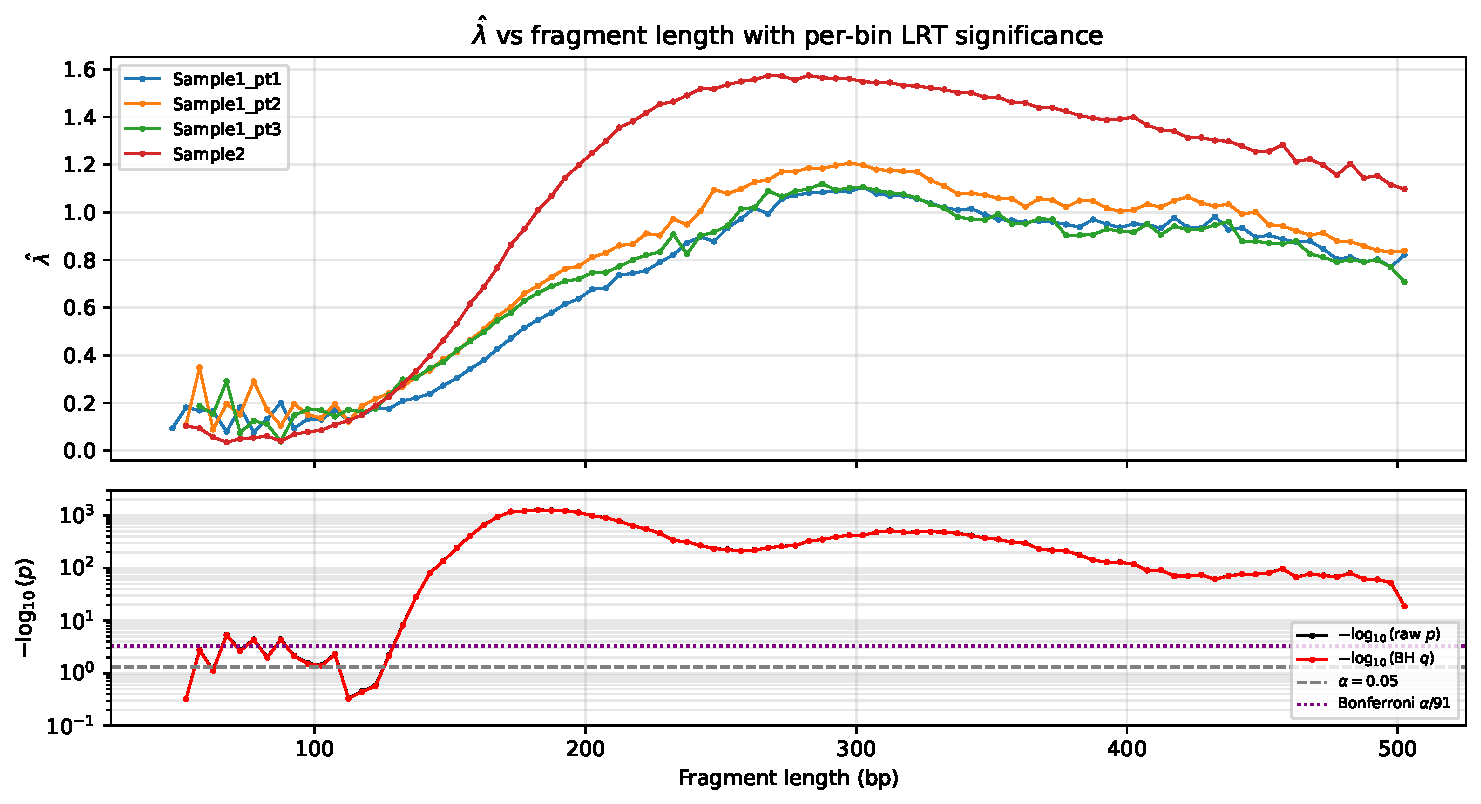
\includegraphics[width=0.95\linewidth]{q3b_lrt.pdf}
\caption{\textbf{Top:} $\hlam_\ell$ vs fragment length, one curve per file.
\textbf{Bottom:} per-bin LRT $-\log_{10}(p)$ (raw $p$ black, BH $q$ red),
log $y$-axis; \textbf{higher = stronger rejection of $H_0$}. Reference lines:
$\alpha = 0.05$ (grey dashed), Bonferroni $\alpha/91$ (purple dotted) -- reject
above either line.}
\label{fig:q3-lrt}
\end{figure}

\paragraph{Per-file summary.}
\begin{center}
\renewcommand{\arraystretch}{1.15}
\begin{tabular}{lrrrr}
\textbf{File} & \textbf{peak $\hlam_\ell$} & \textbf{peak at (bp)} &
\textbf{mean $\hlam_\ell$} & \textbf{retained bins} \\\hline
Sample1\_pt1 & $1.105$ & $302$ & $0.707$ & $92$ \\
Sample1\_pt2 & $1.206$ & $298$ & $0.801$ & $91$ \\
Sample1\_pt3 & $1.119$ & $288$ & $0.738$ & $90$ \\
Sample2      & $1.574$ & $282$ & $1.069$ & $91$ \\
\end{tabular}
\end{center}
The retained length range is $\sim\![48,\, 502]\,\text{bp}$ across all files
(bins with $U_\ell < 50$ discarded). All four peak between $282$ and $302\,\text{bp}$
-- a $20\,\text{bp}$ window -- while peak heights span a much wider range
($1.10$--$1.57$). Mean $\hlam_\ell$ averaged across all bins ranks the files in the
same order as the global $\hlam$ from Q2(a), as expected.

\subsection{(b) Comparing $\lambda(\ell)$ across files; significance}
\emph{Question (Ex2.pdf).} How do these functions differ between the different
sequencing files? How would you assess if they are significantly different?

\paragraph{Patterns visible by eye in Figure~\ref{fig:q3-lrt}.}

\textbf{(P1) Sample~2 sits uniformly $40$--$50\%$ above the Sample~1 parts above
the size-selection cutoff ($\ell \gtrsim 120\,\text{bp}$).} Shape (peak,
asymmetry, decay) is identical; only the amplitude is shifted. Consistent with
deeper per-molecule sequencing at a shared protocol -- Q2(a)'s global $\hlam$
ratio $1.20/0.78 \approx 1.54$ matches the per-length amplitude shift.

\textbf{(P2) The three Sample~1 parts trace nearly the same curve} (within
$\sim 10\%$ in amplitude). A meaningful improvement over Q2(a), where the
global $\hM_{\text{fit}}$ values disagreed by $\sim 60\%$ -- evidence that
length is the dominant heterogeneity axis Q2(b) detected.

\textbf{(P3) The peak location is shared across all four files
($\ell \approx 290\,\text{bp} \pm 10$).} Set by library-prep target insert size
and the PCR sweet spot, both shared across the same protocol (discussed in Q3(c)).

\textbf{(P4) Sample~2 is visibly smoother} because each bin holds $\sim 2\times$
more fragments and the per-bin variance scales as $1/U_\ell$ -- noise, not a
different process.

\paragraph{Formal significance test: the likelihood-ratio test (LRT).}
Compare $H_0$ (all $F = 4$ files share one rate $\lambda_\ell$ at this bin)
against $H_1$ (each file has its own $\lambda_\ell^{(f)}$, $f = 1,\dots,F$).
$H_0$ is nested in $H_1$, so $H_1$ never fits worse; the question is whether
it fits \emph{much} better (real differences) or only marginally (sampling
noise). \emph{Full derivation in the supplementary statistics primer
(\texttt{stats\_primer.pdf}).}

\emph{The statistic.} For each file $f$, the truncated-Poisson log-likelihood derived
in Q1(b) is
\[
   \ell_f(\lambda) \;=\; N_\ell^{(f)} \log \lambda \;-\; U_\ell^{(f)} \lambda
                       \;-\; U_\ell^{(f)} \log\!\bigl(1 - e^{-\lambda}\bigr) \;+\; \text{const.}
\]
The classical \emph{Neyman--Pearson likelihood ratio} for two simple hypotheses
is $\Lambda_{NP} = L(\hat\theta_{H_0}) / L(\hat\theta_{H_1})$ with range
$(0, 1]$, since $L(\hat\theta_{H_1}) \ge L(\hat\theta_{H_0})$ by nesting. We
use the inverted, twice-logged, multi-file form (standard for Wilks):
\[
   \boxed{\;\Lambda_\ell \;=\; 2\Bigl[\, \textstyle\sum_f \ell_f(\hlam_\ell^{(f)}) \;-\; \sum_f \ell_f(\hlam_\ell^{(0)}) \,\Bigr]\;}
\]
where $\hlam_\ell^{(f)}$ is each file's own MLE and $\hlam_\ell^{(0)}$ is the
pooled MLE. By construction $\Lambda_\ell \in [0, \infty)$ -- per file, how
much better fitting its own MLE does than being forced onto the shared one,
summed; \emph{no upper bound}, unlike $\Lambda_{NP}$.

By Wilks' theorem (1938 -- not covered in class), under $H_0$ and mild
regularity, $\Lambda_\ell$ is asymptotically $\chi^{2}$-distributed with
$\mathrm{df} = F - 1 = 3$ (the parameter-count difference, $p_1 - p_0 = F - 1$).
Thus $p_\ell = \Pr\bigl[\chi^{2}(F-1) > \Lambda_\ell\bigr]$.

\paragraph{Multiple-testing correction.}
With $91$ simultaneous tests I apply both corrections discussed in Lecture~5:
\emph{Bonferroni} (controls FWER; threshold $\alpha/91 \approx 5.5\times 10^{-4}$;
safe but conservative) and \emph{Benjamini--Hochberg} (controls FDR; adaptive
step-up procedure rejecting at $p_{(k)} \le (k/91)q$). Reporting both lets the
conclusion be checked for robustness; BH is the more powerful here since
Bonferroni already shows most nulls are false.

\paragraph{Result.}
Running the test on the four files at the $91$ length bins gives:
\begin{center}
\renewcommand{\arraystretch}{1.15}
\begin{tabular}{lrr}
\textbf{Rejection criterion} & \textbf{Bins rejecting $H_0$} & \textbf{Fraction} \\\hline
Raw $p < 0.05$ (no correction)               & $86$ & $95\%$ \\
Benjamini--Hochberg $q < 0.05$ (FDR)         & $86$ & $95\%$ \\
Bonferroni $p < 5.5 \times 10^{-4}$ (FWER)   & $78$ & $86\%$ \\
\end{tabular}
\end{center}
The curves are genuinely different across files, robustly to the choice of
correction. The raw-$p$ and BH-$q$ counts coincide because the LRT $p$-values are
sharply bimodal: each bin's $p$ is either far below any threshold (true rejection,
mostly driven by Sample~2 vs Sample~1) or comfortably above $0.05$ (no signal).
The Bonferroni count is slightly lower because its threshold ($\alpha / 91$) is
about $90\times$ tighter than $0.05$, so a handful of mid-magnitude
$p$-values that BH/raw retain are pushed back into ``not rejected''. The same
overall picture nonetheless holds under every correction: at most lengths the four
files have detectably different rates.

\emph{Why $\sim 95\%$ rejection when the Sample~1 parts are supposed to be
replicates?} Two reasons: \textbf{(a)} the LRT is jointly on all four files,
and the Sample~1 vs Sample~2 amplitude gap (P1) dominates most bins, so most
rejections correctly flag Sample~2; \textbf{(b)} with per-bin $U_\ell$ in the
tens of thousands, even a $10\%$ within-Sample-1 spread is statistically
detectable -- the test correctly says the four $\hlam_\ell$ are not
\emph{exactly} equal, not that the differences are biologically meaningful.
Pairwise S1-only LRTs (not run here) would separate the S1-vs-S2 signal from
S1-internal noise.

\subsection{(c) What the curves say about PCR + sequencing bias}
\emph{Question (Ex2.pdf).} What do these graphs tell you about biases in the
PCR + sequencing process?

The four curves agree on a striking qualitative shape -- a steep rise, a peak near
$\ell \approx 290\,\text{bp}$, and a long slow tail. Each feature has a biological
interpretation.

The shape can be read as three regimes, each with its own mechanism.

\textbf{Short side ($\ell \lesssim 120\,\text{bp}$): size-selection.}
Library prep includes a SPRI / gel size-selection step that physically removes
fragments below $\sim 100$--$150\,\text{bp}$ before sequencing. $\hlam_\ell$ is
small and noisy there because the input is absent, not because PCR failed.

\textbf{Peak ($\ell \approx 290\,\text{bp}$).}
Two reinforcing effects: protocols target a $200$--$400\,\text{bp}$ insert
range so the pre-PCR pool is densest there, and PCR efficiency is highest in
the same range (reliable annealing, fast extension, low fall-off). All four
files peaking at the same length supports a common protocol target.

\textbf{Long side: PCR length bias.}
PCR efficiency declines gradually with length (polymerase fall-off, strand
breaks, harder strand-displacement), geometrically per cycle; after
$\sim 10$--$15$ cycles this accumulates into the slow decay seen here. The
asymmetric shape (steep left, gradual right) is the fingerprint of a physical
cutoff on the short side and a continuous efficiency decline on the long side.

\paragraph{Connection back to Q2(b).}
$\hlam_\ell$ varies by a factor of $\sim 5$--$10$ across length; the global
$\hlam$ from Q1/Q2 averages over this variation, which is why the global
truncated-Poisson fits so badly. Stratifying by length is the natural fix for
this axis of bias.

\subsection{(d) Reconstructing the original fragment-length distribution}

\emph{Question (Ex2.pdf).} Can you reconstruct the presumed fragment-length
distribution in the original library? Explain how you go about it and what
you learned.

\paragraph{Within-bin homogeneity assumption.}
The model below assumes a single $\lambda_\ell$ governs every fragment in length
bin $\ell$. Q3(b) gives indirect support -- the three Sample~1 replicates agree
within $\sim 10\%$ at every bin, consistent with one common per-bin rate -- but
this is not a goodness-of-fit test. A formal check (per-bin Pearson $\chi^{2}$,
as in Q2(b)) is not asked for and was not run, so the $\hM_\ell$ below inherit
whatever within-bin heterogeneity persists.

\paragraph{Method.}
Per length bin $\ell$, the truncated-Poisson model says
\[
   \E[U_\ell] \;=\; M_\ell \bigl(1 - e^{-\lambda_\ell}\bigr),
\]
where $M_\ell$ is the (unknown) pre-PCR molecule count at length $\ell$.
Substituting the observed $U_\ell$ for $\E[U_\ell]$ and $\hlam_\ell$ from Q3(a),
\[
   \hM_\ell \;\approx\; \frac{U_\ell}{1 - e^{-\hlam_\ell}} \;=\; \frac{N_\ell}{\hlam_\ell}
\]
(the second equality holds at the MLE, by the same algebra as Q1(d) and the
Setup of Q2).

\paragraph{Why dividing by $(1-e^{-\hlam_\ell})$ undoes the length bias.}
Q3(a)--(c) established that $\hlam_\ell$ is not flat: it peaks near
$290\,\text{bp}$ -- PCR's sweet spot -- and falls off in both directions.
Consequently the detection probability $(1 - e^{-\hlam_\ell})$ is also
length-dependent: high (close to $1$) at lengths PCR amplifies well, lower (down
to near $0.4$) at lengths it does not. Because $\E[U_\ell] = M_\ell (1 -
e^{-\lambda_\ell})$, the un-normalised observed count $U_\ell$ already mixes the
true abundance $M_\ell$ with the length-dependent detection probability -- so a
raw histogram of $U_\ell$ is biased toward lengths PCR favours. Dividing by the
\emph{same length-specific} detection probability removes that mixing factor:
$\E[U_\ell / (1 - e^{-\lambda_\ell})] = M_\ell$, i.e.\ the estimator is
\emph{unbiased} for the pre-PCR count $M_\ell$ in the statistical sense that its
expected value equals the parameter. Bins PCR over-amplified get a near-$1$
correction; bins it neglected get a large boost that recovers (in expectation)
the silent molecules that produced zero reads.

\emph{Is this enough?} It is sufficient to invert the length axis of the bias.
It is \emph{not} a guarantee that all PCR-induced distortion vanishes: any
heterogeneity orthogonal to length -- GC content, sequence context, mappability,
position effects -- is not corrected by this inversion and remains baked into
$\hM_\ell$. The estimator returns the pre-PCR length distribution that is
consistent with treating length as the dominant bias axis, not absolute molecule
counts. See \emph{Sufficiency check} below for an empirical test of how much
the correction actually achieves on these data.

\paragraph{Normalising.}
The normalised sequence $\hat{p}_\ell^{\text{(pre)}} = \hM_\ell /
\sum_{\ell'} \hM_{\ell'}$ is a probability distribution -- the fraction of the
pre-PCR library at each length, with the library-size scale divided out so files
of different total sizes are comparable. The raw observed
$\hat{p}_\ell^{\text{(obs)}} = U_\ell / \sum U_{\ell'}$ is computed alongside as
the post-PCR baseline.

\paragraph{Implementation.}
\texttt{q3d.py} extends \texttt{q3a.py} with the per-bin $\hM_\ell$ and the
normalised distributions $\hat{p}_\ell^{\text{(pre)}}$ and
$\hat{p}_\ell^{\text{(obs)}}$, computes per-distribution summary statistics, and
runs the sufficiency check below.

\paragraph{Results.}
\begin{center}
\renewcommand{\arraystretch}{1.15}
\setlength{\tabcolsep}{4pt}
\begin{tabular}{l rrrrr @{\hspace{1.2em}} rrrrr}
\toprule
 & \multicolumn{5}{c}{\textbf{Observed $\hat p^{(\text{obs})}_\ell$ (post-PCR)}}
 & \multicolumn{5}{c}{\textbf{Reconstructed $\hat p^{(\text{pre})}_\ell$ (pre-PCR)}} \\
\cmidrule(lr){2-6}\cmidrule(lr){7-11}
\textbf{File}
 & peak & mean & med. & std & IQR
 & peak & mean & med. & std & IQR \\
\midrule
Sample1\_pt1 & $178$ & $258$ & $208$ & $97$ & $153$ & $168$ & $232$ & $180$ & $94$ & $144$ \\
Sample1\_pt2 & $168$ & $252$ & $196$ & $96$ & $151$ & $168$ & $233$ & $181$ & $94$ & $145$ \\
Sample1\_pt3 & $168$ & $253$ & $198$ & $96$ & $152$ & $168$ & $235$ & $182$ & $95$ & $146$ \\
Sample2      & $182$ & $243$ & $224$ & $85$ & $116$ & $\mathbf{142}$ & $\mathbf{206}$ & $\mathbf{181}$ & $92$ & $121$ \\
\bottomrule
\end{tabular}
\end{center}
All units bp; lengths are bin midpoints. Two patterns stand out.

\textbf{(i) The reconstructed distribution sits to the left of the observed
one,} on every statistic: peak drops by $0$--$40\,\text{bp}$, mean by
$17$--$37\,\text{bp}$, median by $0$--$43\,\text{bp}$. This is the PCR-bias
correction working as intended -- $\hlam_\ell$ peaks near
$\ell \approx 290\,\text{bp}$, so fragments in that range are over-represented
in $U_\ell$; dividing by $(1 - e^{-\hlam_\ell})$ pulls probability mass back
toward the short end where the underlying library has more molecules per read.

\textbf{(ii) Sample~2's shift is much larger than Sample~1's.}
Sample~2 has uniformly higher $\hlam_\ell$ (Q3(b)), so its absolute correction
factor $1/(1-e^{-\hlam_\ell})$ is closer to $1$ everywhere; but the peak
location is set by the \emph{relative} shape of the correction across bins. The
relative shape pulls Sample~2 from $182 \to 142\,\text{bp}$; the three Sample~1
parts share a different relative shape that leaves the peak at $168\,\text{bp}$.
After correction, however, the median converges -- $180$--$182\,\text{bp}$ for
all four files -- which is exactly the cfDNA signature (see biological reading
below).

\begin{figure}[!htbp]
\centering
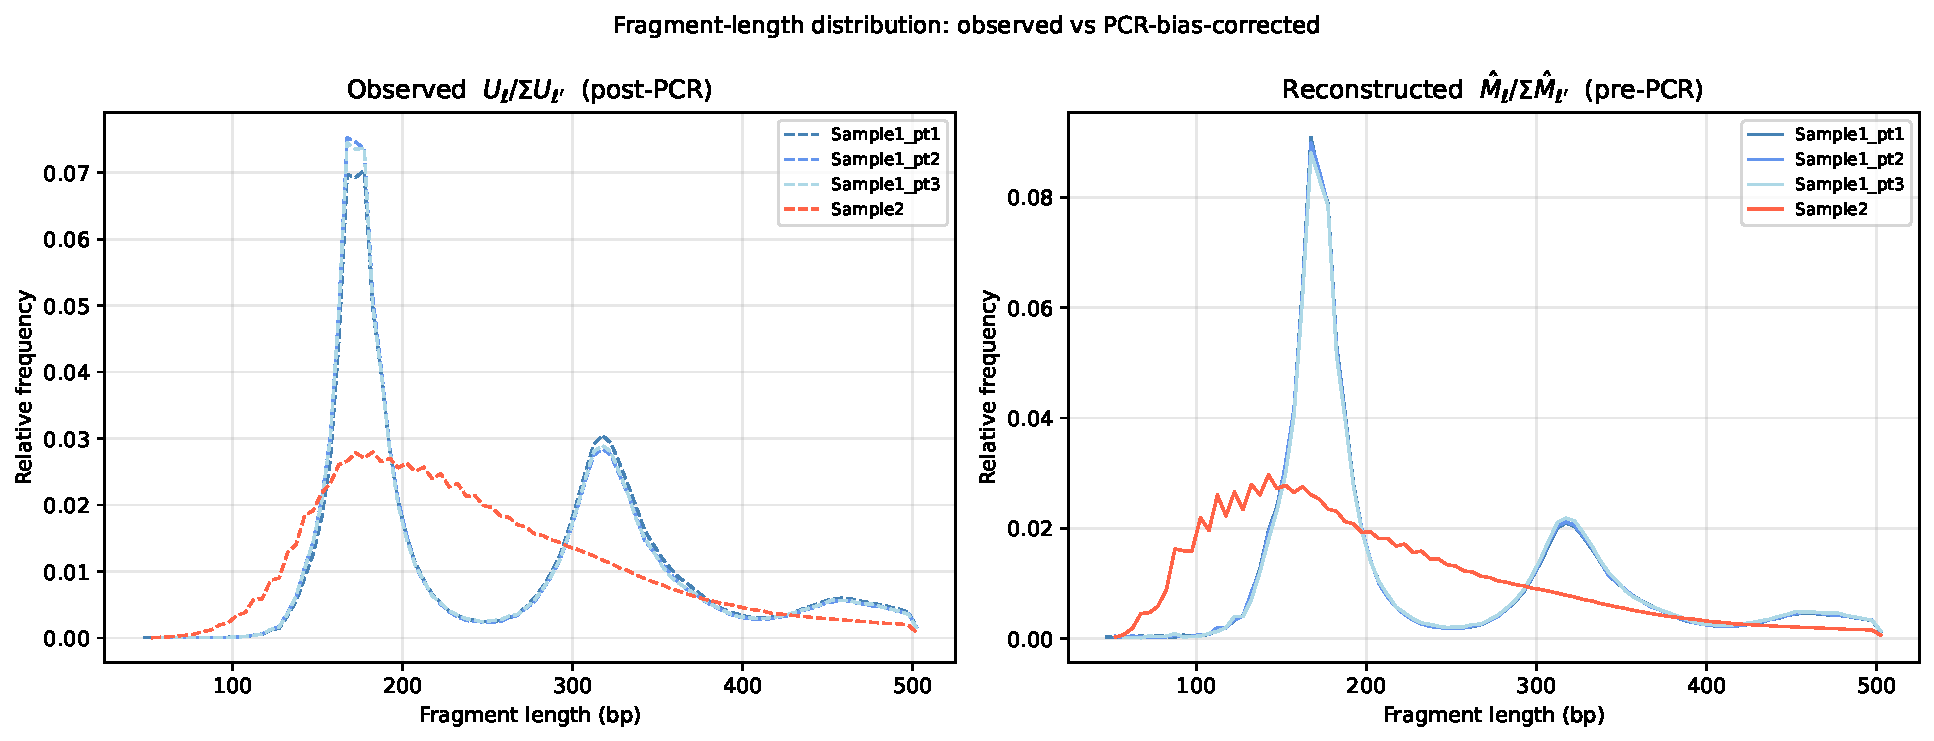
\includegraphics[width=\linewidth]{q3d_length_distribution.pdf}
\caption[Fragment-length distribution before and after PCR-bias correction.]%
{Fragment-length distribution before and after PCR-bias correction.
\textbf{Left:} raw observed distribution
$\hat{p}_\ell^{\text{(obs)}} = U_\ell / \sum U_{\ell'}$ -- biased toward the PCR
sweet spot near $\ell \approx 290\,\text{bp}$.
\textbf{Right:} reconstructed pre-PCR distribution
$\hat{p}_\ell^{\text{(pre)}} = \hM_\ell / \sum \hM_{\ell'}$, dividing through by
the per-bin detection probability $(1 - e^{-\hlam_\ell})$. The dominant peak
near $\ell \approx 168\,\text{bp}$ and the secondary shoulder near
$\ell \approx 320\,\text{bp}$ persist in both panels.}
\label{fig:q3d-length-dist}
\end{figure}

\paragraph{Biological reading: why two peaks, not one.}
The reconstructed distribution has a dominant peak near $168\,\text{bp}$
(Sample~1) or $142\,\text{bp}$ (Sample~2) and a secondary shoulder near
$320\,\text{bp}$ that survives the correction. This is the classic cell-free DNA
fragmentation pattern: cfDNA is preferentially cleaved in nucleosome linker
regions, leaving fragments at integer multiples of the $\sim 167\,\text{bp}$
nucleosome footprint -- a sharp mono-nucleosome peak and a di-nucleosome shoulder
near $\sim 330\,\text{bp}$. The presence of \emph{both} peaks after correction
indicates they are not PCR artefacts but real features of the input library.
Sample~2's sharper, shorter peak ($142$ vs $168\,\text{bp}$, smaller IQR) is
consistent with a more degraded or differently-prepared cfDNA library.

\paragraph{Sufficiency check.}
A free internal test of whether the correction does anything useful: the three
Sample~1 parts are presumed replicates of one library, so their reconstructed
distributions should agree more closely than their observed distributions. Using
total variation distance ($\TVD$),
\begin{center}
\renewcommand{\arraystretch}{1.1}
\begin{tabular}{lrrr}
\textbf{Pair} & $\TVD$ \textbf{(obs)} & $\TVD$ \textbf{(pre)} & \textbf{change} \\\hline
pt1 vs pt2 & $0.032$ & $0.008$ & $-0.024$ \\
pt1 vs pt3 & $0.028$ & $0.019$ & $-0.009$ \\
pt2 vs pt3 & $0.008$ & $0.015$ & $+0.007$ \\
\end{tabular}
\end{center}
Two of three pairs move closer; the average $\TVD$ across the three pairs drops
from $0.023$ to $0.014$ ($\sim 40\%$ reduction). The pt2--pt3 pair was already
the closest in observed space, so its slight regression is within the noise of
the per-bin $\hlam_\ell$ estimates. Net: the correction provides a measurable
but partial improvement in replicate consistency, which is what one expects if
length is one important but not exhaustive bias axis.

\emph{Direction-correct, magnitude unverifiable.} The $\TVD$ check says
$\hat M_\ell$ moves the right way, but can't tell under- from over-correction:
within-bin heterogeneity could leave residual PCR bias in $\hat M_\ell$, and
multiplying $1/(1-e^{-\hlam_\ell})$ into low-$\hlam$ bins driven by
size-selection (not PCR inefficiency) could fabricate a left-edge bump. Without
a ground-truth pre-PCR distribution the absolute magnitude is unverifiable.

\paragraph{What we learned.}
(1) The pre-PCR length distribution is recovered by $\hM_\ell =
U_\ell/(1-e^{-\hlam_\ell})$. (2) After correction all four files share a median
near $180\,\text{bp}$ -- the mono-nucleosome footprint -- with a
di-nucleosome shoulder near $\sim 320\,\text{bp}$, consistent with a cfDNA
library. (3) The correction tightens Sample~1 replicate agreement by $\sim 40\%$
in $\TVD$, so length is real but not the only bias axis. Size selection itself
is not invertible -- the small $U_\ell$ at $\ell \lesssim 100\,\text{bp}$
reflects fragments physically removed before sequencing, which no inversion can
recover -- and Q2(b)'s rejection of the global Poisson means absolute molecule
counts would still need other axes (GC, context, position) modelled in.

\end{document}
